\section{Durchführung}
\label{sec:durchfuehrung}
Die Zerfälle werden mit einem Geiger-Müller-Zählrohr detektiert und in einem
Zählwerk erfasst.
Die gezählte Anzahl an Zerfällen wird wechelweise in zwei Anzeigefenstern angezeigt.
Die angergte Probe kann um das Zählrohr gelegt werden, umgekehrt zur Skizze,
insgesamt sind Probe und Zählrohr während der Messung in einer Bleiabschirmung.

\begin{figure}
      \centering
      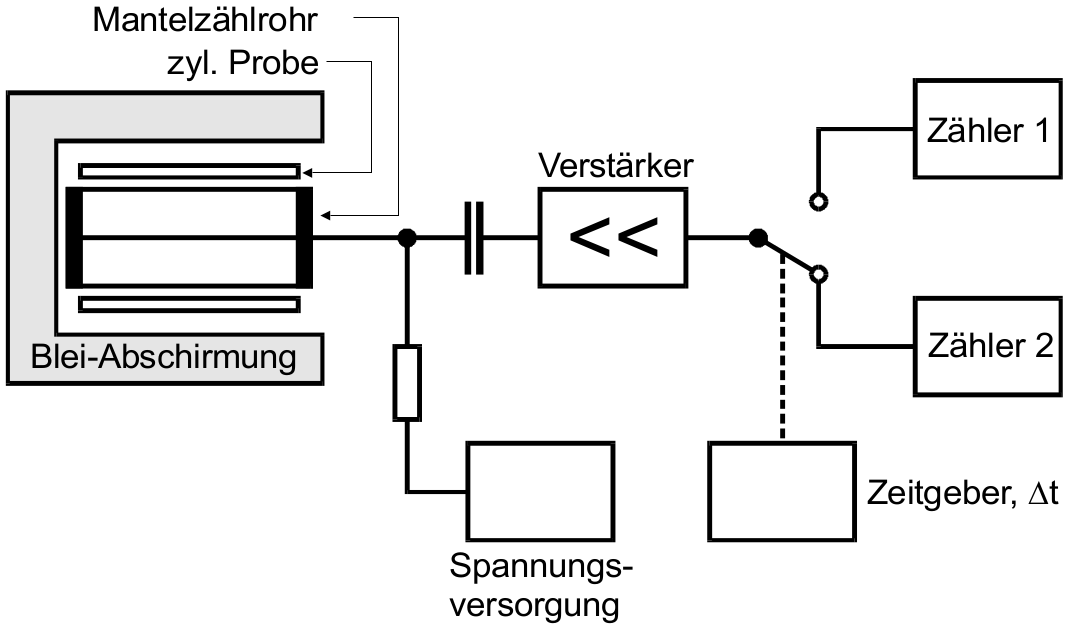
\includegraphics[width=0.7\textwidth]{content/schematischer-aufbau.png}
      \caption{Aufbau des Versuches aus \cite{Anleitung}.}
      \label{fig:aufbau}
\end{figure}

Der systematische Fehler der durch das Wechseln des Zählabschnitts entsteht,
wird aufgrund der dafür benötigten Zeit von etwa $\SI{e-7}{\second}$ im Vergleich
zu den Intervallzeiten in Tabelle \ref{tab:messparameter} vernachlässigt.

Als erstes wird eine Nullmessung durchgeführt, um die allgeneine
Strahlungsintensität herauszufinden, es wird über eine Zeit von
$\SI{800}{\second}$ gemessen.\\
Die Messzeiten der Präparatsmessungen werden einer ausliegenden Tabelle
entnommen. Unsere Messparameter stehen in Tabelle \ref{tab:messparameter},
vgl Kapitel \ref{sec:messmethode}.

\begin{table}
    \centering
    \caption{Messparamter nach ausliegender Tabelle.}
    \label{tab:messparameter}
    \begin{tabular}{c c c}
        \toprule
        & {Indium} & {Rhodium} \\
        \midrule
        {min. Messzeit} & $\SI{60}{\minute}$ & $\SI{12}{\minute}$ \\
        $\increment t$ & $\SI{240}{\second}$ & $\SI{20}{\second}$ \\
        {\# Messwerte} & 36 & 15 \\
        \bottomrule
    \end{tabular}
\end{table}
